% vim: set tw=78 sts=2 sw=2 ts=8 aw et ai:

\chapter{Optimizing deployment}\label{ch:optimizations}
\bigskip

The goal is to provide students an easy to use infrastructure, that
provides good permanence and still remain easy to deploy and maintain.

The following chapter will discuss different approaches tested, with
their pros and cons.

\section{The centralized virtual machine server experiment}

\subsection{Idea and implementation}
Starting with the desire to eliminate the need for operating system
multiplication and system freezing in order to keep images identical, a
push was made to make better use of virtual machines.

To replace the freezing of the workstation's operating system, the
\emph{snapshot} feature of VMware Workstation and VirtualBox would be
used. All the virtual machines would be deployed with a snapshot made.
Before a lab, each student would have to manually revert to the
snapshot and this way all students will have the same working
environment.

But there are a couple of problems with this initial idea. First, if the
physical system is not frozen, a student could delete by mistake the
virtual machine or the snapshot, because the student would have full
control of the physical system's operating system.

There is also the problem with the initial deployment of the virtual
machines to all the workstations so this would also need a network
imaging (using UDPCast).

Another problem is the fact that not all workstations would have the
hardware resources to run virtual machines that would provide students
with a quality experience.

The decision was made to try a centralized approach, where a special
server would be installed and host all the virtual machines. This server
was a Intel Xeon with 8 cores and 16GB of RAM as was supposed to hold 20
virtual machines. The server was running \emph{Vmware vSphere}
hypervisor.

The students would remotely connect to the central virtual machine
server and access their machine from a pool of about 20 machines. Each
group of students would revert to a previous snapshot.

This model would fix some problems. Having a central server, accessed
with user credentials, access control was implemented. Remote users were
able to access the machine, use it, revert snapshots, but not delete the
machines or the snapshots.

The multiplication of the machines was now easy, because it was just a
matter of copying machines on the local server, on the local harddrive,
not over the network.

The idea was not without problems. First of all, the machine was a
single point of failure. If the server would malfunction, no student
would be able to access any virtual machine.

The scalability of the architecture was challenged by the fact that the
server itself was an expensive resource. If you have one server per
room, you need as many servers as rooms.

The challenge was now to see how many virtual machines (full
virtualized) could be instantiated on a machine. A research was made to
test virtualization solutions.

\subsection{Testing Environment}

All the tests were done on a workstation with a Core2Duo E7600 Processor
at 3.06 GHz with Intel VT support. The system had 2GB of physical memory,
320 GB SATA2 hard drive at 7200 RPM and a Gigavit Ethernet network card.
The operating system installed on the system was Ubuntu 10.4.2 runnning
Linux kernel 2.6.32 with KVM support.

\subsection{VMware Workstation}

The first virtualization solution tested was VMWare Workstaiton 7.2.
Although the Workstation products from VMware are not designed to run a
large number of virtual machines on a single physical host, it is one of
the most popular and advanced virtualization solution and was tested to get
a benchmark for comparison.

An virtual machine was created being allowed the use of one processor and
512 MB of RAM. It was set up to boot a live CD from an Ubuntu 11.04 iso
file. 10 Clones were made using the \emph{vmrun} command line tool and were
started simultaneous. This first test monitored the time needed for the
LiveCD distribution to boot up from power on until it reaches an idle state
waiting for user input. It was a stress test to see how the solution scales
under concurrent load and the results were there for comparison with the
QEMU-KVM solution.

The boot-up of a single machine into the Ubuntu Live CD took about 60
seconds and boot-up of two simultaneous images took the same time (the
system had two cores and more physical memory than the sum of the
virtualized memory). 3 Simultaneous boot-ups took 100 seconds. When booting
4 clones, 3 minutes were needed to reach the benchmark state, but started
causing serious performance problems for the host machine. Booting 5 or
more clones made the host system completely freeze.

Further testings were not made and the solution was not chosen because of
the lack of scalability it provides and also because VMware Workstation is
not either free nor open source and the licence for the use is expensive.

Enterprise solutions that would scale to a large number of virtual machines
in the wanted environment would be VMware ESX or Microsoft Hyper-V, but
they are also not choses because of the high financial cost.

\subsection{QEMU-KVM}


The main tests were done the QEMU with KVM support framework. A simple
deployment of KVM and Qemu requires processor with hardware virtualization
support (such was the case with the Intel Core2Duo CPU used) and  Linux
kernel with KVM support. Userspace packets were also needed to provide
command line and GUI tools.

As the VMware test before, virtual machines were allowed 512MB of RAM to be
used and were made to boot an Ubuntu 11.04 Live CD.

Booting one ore two instances of the LiveCD at the same time took about 40
seconds while booting 3 instances took 60 seconds and 4 instances 120
seconds. When booting 5 instances, the needed time was 4 minutes and the
host system started being affected in usability. Launching more instances
severely slowed both guests and host machines but no crashes were reported.
QEMU does not block the execution of more machines if there are not enough
resources available (unlike VMware that doesn't start machines if there is
not enough RAM).

Here are the compared results of VMware and QEMU-KVM  of boot-up time of
the same LiveCD distribution under same conditions:


\begin{table}
\begin{tabular}{|l|l|l|}
\hline
\multicolumn{3}{|c|}{Boot-up time (secconds)} \\
\hline
No. of VM & VMware & QEMU-KVM \\ \hline
1 & 60 & 40 \\
2 & 60 & 40 \\
3 & 100 & 60 \\
4 & 180 & 120 \\
5 & freeze & 240\\
\hline
\end{tabular}
\caption{VMware vs QEMU-KVM VM bootup time comparison}
\label{table:virt_bootup_time_comparison}
\end{table}



the next tests made tested the scalability of QEMU-KVM by analysing the
time overhead introduced when running multiple machines under tree heavy
operations: input-output intensive operations (IO), processor intensive
operations (CPU), and network intensive operations (Net).

To do this, tree scripts were created, scripts what simulated the needed
conditions. Each of them got the running duration by the use of the
\emph{time} command. The scripts were ran remotely with the use of
\emph{ssh}.

IO was tested with the use of the \emph{dd} tool that copied
128MB or random data from /dev/urandom to a local file. 

\begin{verbatim}
#!/bin/bash
echo "Testing IO speed"
time (dd if=/dev/urandom of=random.dd \
	bs=1MB count=128 2>/dev/null)
rm random.dd

\end{verbatim}

Intensive CPU was tested with the use a Python scrips that calculates the
value of PI using a statistic method.

\begin{verbatim}
#!/bin/bash
echo "Testing computation speed"
# pi.py calculates value of Pi
# using a statistic method
time (python pi.py \
	2>/dev/null)
\end{verbatim}

Network operations was tested by downloading a ~60 MB file from the
Internet with the \emph{wget} tool.

\begin{verbatim}
#!/bin/bash
echo "Testing network (Internet) speed"
time (wget \
	http://cdimage.debian.org/\
	debian-cd/6.0.1a/i386/iso-cd/\
	debian-6.0.1a-i386-netinst.iso\
	2>/dev/null)
rm debian-6.0.1a-i386-netinst.iso
\end{verbatim}

The tests were ran on up to 10 QEMU-KVM machines running Debian 6.0
(installed only with CLI). Each machine used maximum 512 MB of RAM, one
virtual CPU and a 8GB virtual hard drive.  The virtual network interfaces
were behind a local NAT of the host. The machines were cloned from an
initial machine.

Each of the three tests were executed on the machines that were in idle
state. First set of tests were ran simultaneous on one virtual machine, the
next on two machines and so on, up to all 10 machines. The times from each
execution was collected. The table below, shows the average time of the
executions:

\begin{table}
\begin{tabular}{|l|l|l|l|}
\hline
\multicolumn{4}{|c|}{Operation duration (secconds)} \\
\hline
No. of VM & IO & CPU & Network \\
\hline
0 (physical host) & 18 & 12 & 20\\
\hline
 1 & 19 & 13 & 22\\
 2 & 25 & 17 & 40\\
 3 & 37 & 23 & 57\\
 4 & 50 & 33 & 77\\
 5 & 61 & 43 & 96\\
 6 & 74 & 48 & 112\\
 7 & 87 & 57 & 140\\
 8 & 99 & 67 & 148\\
 9 & 125& 82 & 160\\
10 & 125& 93 & 171\\
\hline
\end{tabular}
\caption{VMware vs QEMU-KVM VM performance comparison}
\label{table:virt_performance_comparison}
\end{table}



Charts were plotted based on the data retrieved to see what is slow down
cause by running several virtual machines at once. By analysing the
evolution of the overhead, we can estimate the scalability of the QEMU-KVM
solution.


\begin{figure}[ht]
\begin{center}
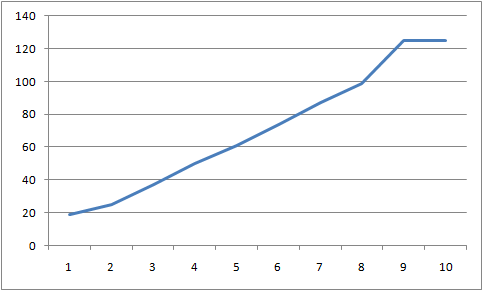
\includegraphics[scale=0.5]{img/io}
\end{center}
\caption{QEMU-KVM Scalability - IO overhead}
\label{fig1}
\end{figure}
\begin{figure}[ht]
\begin{center}
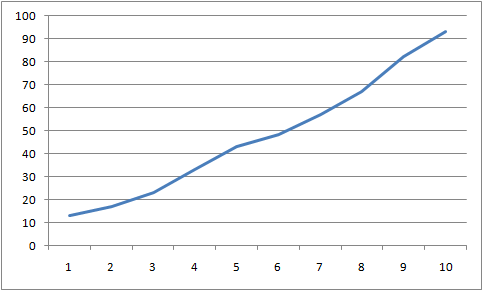
\includegraphics[scale=0.5]{img/cpu}
\end{center}
\caption{QEMU-KVM Scalability - CPU overhead}
\label{fig2}
\end{figure}
\begin{figure}[ht]
\begin{center}
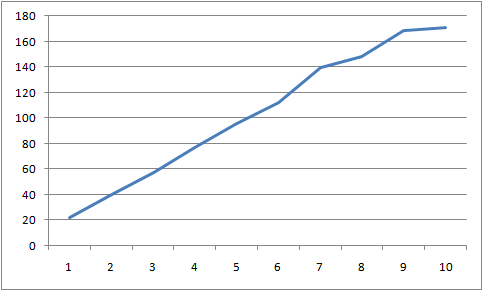
\includegraphics[scale=0.5]{img/net}
\end{center}
\caption{QEMU-KVM Scalability - Network overhead}
\label{fig3}
\end{figure}


\subsection{Experiment conclusions}

Although a central virtual machine server would be more efficient from
an administration and deployment point of view, the costs outweigh the
benefits. Neither the open source KVM solution nor the enterprise VMware
vSphere solution could provide enough virtual machines instances per
physical machine in order to scale.

A single server powerful enough to host 20+ machines is too expensive
compared to other approaches. A cluster of cheaper workstations would be
more cost effective, but still not scale to the required number of
virtual machines needed.

The model was discarded after one semester.


\section{Replacing freezing with LiveCDs}


Freezing of the operating system system is commonly found with LiveCD
(LiveDVD, LiveUSB) Linux distributions. So another idea was to use
LiveCDs instead of a distribution installed on the local hard drive.

But using actual CDs or DVDs was not a good proposal for several
reasons. First, not all workstations have CD/DVD drives and using
\ac{USB} sticks is expensive. Moreover, booting from such device takes
longed than from the hard disk.

Booting LiveCD ISO images off the network using \ac{PXE} would be an
alternative, but, as discussed in previous chapter, PXE has its
drawbacks.

An new idea related to Live distribution booting came along with version
2 of \ac{GRUB}. Grub2 is the next generation Linux bootloader that is
trying to replace the “Legacy” Grub version. It is a complete rewrite of
Grub 1 and only lately becoming fully featured compared to the old
version and even comes with some new interesting features.


An useful new feature in Grub2 is the possibility to boot from an ISO
file. A LiveCD can be stored in an .iso file on disk and loaded by
Grub without having to burn it onto CD or having to boot the normal
system first. A menu entry for ISO booting would look like this:


\begin{verbatim}
menuentry "Ubuntu LiveCD" {
        loopback loop (hd0,1)/boot/iso/ubuntu-12.04-desktop-i386.iso
        linux (loop)/casper/vmlinuz boot=casper
:iso-scan/filename=/boot/iso/ubuntu-12.04-desktop-i386.iso noprompt
noeject
        initrd (loop)/casper/initrd.lz
}
\end{verbatim}

What this feature provides is the possibility of providing a contained
environment (similarly to a friezed system) but stored on the hard disk.
Students could transparently boot the distribution without knowing it's
actually a LiveCD.

If virtual machines or virtual containers are required, they could be
bundled up in a custom Live image packet in a new iso file.

\section{Syncing over the network}

The previous idea, with booting live distributions from iso files on the
disk does replace the need for system freezing, but still needs a
deployment mechanism.

Using UDPcast to copy the disk images to all the stations would also
copy the iso images on the disk. But since now the operating system is
packet inside a single (iso) file rather than on a partition or an
entire disk, we could use other network transfer protocols to copy
files.

\emph{SAMBA} is a good protocol that allows file sharing on the
\ac{LAN}. Better protocols for the given situation is \emph{rsync} or
\emph{\ac{NFS}}. The later two provide a synchronization mechanism
between two sources.


\section{Using Intel vPro technology}


Starting with the its Core 2 processors series, Intel introduced the
\emph{vPro technology}. vPro is an umbrella term for a series of
hardware technologies built into computer chips produced by Intel, among
which, \emph{Intel’s Active Management Technology (AMT)}. The \ac{AMT}
technology allows remote management features to computers that use vPro
processors in order to monitor, maintain, and manage the target computer
regardless of the Operating System (or regardless of the existence of an
Operating System) or its power state. \ac{AMT} and vPro also introduce
security features such as remote shutdown of computers in case of theft.

A description of vPro is available in Whitepaper \cite{paper:intel-vpro}
released by Intel corporation, cited here.

Desktop PCs with Intel® vPro™ technology provide built-in, professional-
grade management and security capabilities that meet critical business
challenges. IT can lower maintenance costs while ensuring greater levels
of IT compliance using Intel vPro technology’s improved remote
management, provisioning, problem resolution, off-hours maintenance, and
proactive security capabilities—all directly from the IT console.

Most importantly, these hardware-based capabilities are available to
authorized IT down-the-wire, even for PCs that are powered off or whose
operating system (OS) is down. IT will now be able to remotely take
accurate asset and hardware/software inventories, contain more security
threats, resolve software and hardware problems faster, and increase
user uptime.

PCs with Intel vPro technology also include additional,
hardware-based capabilities that give IT the option of a lighter-weight
form of virtualization for mainstream business. IT can now run critical
security applications in a simplified, self-contained, dedicated virtual
partition—or “virtual appliance” even while users are working on their
own compute-intensive tasks in the user OS.

These powerful new hardware-based capabilities are designed right into
PCs with Intel vPro technology. And, every PC with Intel vPro technology
uses the Intel® Core™2 Duo processor. The Intel Core 2 Duo processor
gives IT the dual-core, 64-bit capable performance needed to run the
latest compute-intensive applications and provide outstanding user
responsive ness in multitasking environments—all in a power-efficient
design that is Windows Vista* Premium Ready. IT can now spend less time
on routine tasks, and can focus resources where they are most needed for
better manageability and security of desktop PCs.

\subsection{Remote node management}

The \ac{AMT} technology allows for active discovery of the workstations
in the network and then access that workstation using \ac{VNC}. Because
of the built in TCP/IP stack, the workstation will have IP connectivity
even if there is no operating system available.

The control is made via the open standard \ac{VNC} so this means that I
can be controlled by any client running this protocol.

\begin{figure}[ht]
\begin{center}
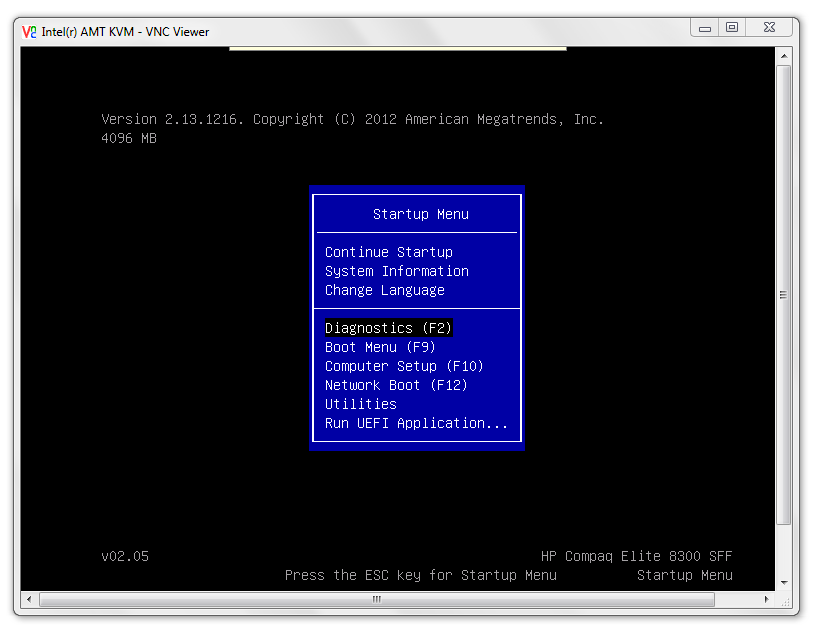
\includegraphics[scale=0.5]{img/intel_amt_bios}
\end{center}
\caption{Accessing BIOS on remote workstation with Intel AMT}
\label{fig1}
\end{figure}


\subsection{Remote ISO boot}


A more relevant feature for the purpose of this thesis is the
\emph{Remote ISO Launcher}. Intel releases a proof-of-concept software
that uses the \ac{AMT} framework, under open source licence. The Remote
ISO Launcher can connect to a remote workstation and transfer via the
network connection an iso image and make the workstation boot the Live
from the network.

This is similar to what \ac{PXE} could do, but \ac{AMT} uses a push,
rather than a pull model. In PXE, the client workstation would as a
\ac{TFTP} server for an image  and boot from it, starting with the
kernel. In AMT, a central station, running the Remote ISO Launcher will
control the remote node, restart it, push the image to it and the client
node would boot. In the second case, at no time would the administer
need to be in front of the client workstation.

At the time of writing this thesis, the version of Remote ISO Launcher
offers just basic operations (like rebooting the remote machine and
booting the ISO). But the API of AMT offers a larger number of
operations (for example, the ability to run commands on the remote
operating system after boot time).

Being open source, the Remote ISO Launcher could be extended to offer
features like sending reboot commands periodically to restart the
operating system, shut down the target computer in off-hours or
scheduling certain images to be load at wanted hours.


